\documentclass[a4paper]{article}

\usepackage{fullpage}
\usepackage{amsmath}
\usepackage{amsthm}
\usepackage{amssymb}
\usepackage{listings}
\usepackage{parcolumns}
\usepackage{graphicx}
\usepackage{todonotes}
\usepackage{tlaops}
\usepackage{tlaplus}

\title{An instantiation algorithm for TLA+ expressions}
\author{}


\theoremstyle{definition}
\newtheorem{theorem}{Theorem}[section]
\newtheorem{lemma}{Lemma}
\newtheorem{definition}{Definition}

\newcommand{\sidebyside}[2]{
  \begin{minipage}{0.45\linewidth}
    #1
  \end{minipage}
  \hspace{10pt}
  \begin{minipage}{0.45\linewidth}
    #2
  \end{minipage}
}

% \newcommand{\parsbs}[2]{
% \begin{parcolumns}{2}
%   \colchunk{
%     {#1}
%   }
%
%   \colchunk{
%     {#2}
%   }
% \end{parcolumns}
% }

\lstdefinelanguage{tlaplus}{
  morekeywords= { MODULE, LET, IN, VARIABLE, VARIABLES, CONSTANT, CONSTANTS,
    ASSUME, NEW, PROVE, THEOREM, LEMMA, ENABLED, ==, INSTANCE, BY, DEF, QED,
    TAKE, HAVE, SUFFICES, PICK },
  sensitive=true,
  morecomment=[l]{\*},
  morecomment=[s]{(*}{*)},
  morestring=[b]",
  literate={~} {$\sim$}{1},
  columns=fullflexible,
  basicstyle=\small
}

\lstset{language=tlaplus}

\begin{document}

\maketitle

\section{Overview}
\label{sec:overview}
\tlaplus{} has two kinds of substitution: instantiation of modules, which
preserves validity, and beta-reduction of lambda-expressions, which does not
necessarily preserve validity. Following the notions of SANY, we distinguish
three kinds of variables: temporal constants and temporal variables are
bound by instantiation whereas formal parameters are bound by lambda
abstraction. Furthermore, ENABLED binds all temporal variables within its
argument which are in the context of the next state operator '.

In the presence of unresolved instantiations or substitutions, it is often
unclear, which operator binds the occurrence of a particular temporal variable:
when we consider the expression
\tla{$(\lambda\; fp : ENABLED\; (fp \dif fp'))(x)$}, it seems that the variable
$x$ is bound in the module. But in the beta-reduced form $ENABLED\; (x \dif x')$
of this expression, only the first occurrence of $x$ is bound by the
module but its second (primed) occurrence is bound by ENABLED\footnote{To
  prevent complications from renaming, we will not assume alpha equivalence but
  will handle the renaming of bound variables explicitly.}.

Furthermore, the two substitutions do not commute. For example, let us
consider modules Foo and Bar:

\begin{parcolumns}{2}
  \colchunk{
    \begin{lstlisting}
      ---- MODULE Foo ----

      VARIABLE x

      E(u) == x' # u'
      D(u) == ENABLED ( E(u) )

      THEOREM T1 == D(x)

      ====
    \end{lstlisting}
  }
  \colchunk{
    \begin{lstlisting}
      ---- MODULE Bar ----

      VARIABLE y

      I == INSTANCE Foo with x <- y


      THEOREM T2 == I!D(y)

      ====
    \end{lstlisting}
  }
\end{parcolumns}

\vspace{2mm}
\noindent
It looks like \tla{I!T1} and \tla{T2} talk about the same formula \tla{D(y)},
but this is not the case: the first can be read as \tla{I!(D(y))}\footnote{This
  is not valid \tlaplus{} syntax.} and the second as \tla{(I!D)(y)}. In other
words, it makes a difference if we beta-reduce first or if we instantiate
first. Reducing D(x) first leads to \tla{ENABLED (x' \dif x')}, which --
following the renaming instuctions in ``Specifying Systems'' -- becomes
\tla{ENABLED (\$x' \dif \$x')} by the instantiation of \tla{x} with \tla{y},
because primed occurrences of \tla{\$x} are bound by their enclosing ENABLED,
not by the instantiation.

Instantiating first keeps the occurrence of the  formal parameter \tla{u} intact,
leading to \tla{I!D(u) == ENABLED ( u \dif \$x') } but reducing the application
\tla{I!D(y)} leads to \tla{ENABLED (y' \dif \$x')}. Now it is clear that
\tla{I!(D(y))} is unsatisfiable while \tla{(I!D)(y)} is valid.\footnote{ Since
  one of the axioms  of \tlaplus{} is that (TRUE \dif FALSE), we can always find
  a domain element different from $x$. In fact, the axioms of set-theory even
  enforce denumerable models.}.

In the following, we will develop algorithms for both kinds of substitutions.
Since the occurrence of a lambda reducible expression (redex) as a subterm of
an instantiation may block the evaluation of the latter, inner substitutions
(i.e. those closer to the leaves of the term tree) must be evaluated before
outer ones. Definitions will also need special consideration because
we allow some of them to stay folded. But since a definition can contain
substitutions, they can not be treated like temporal constants.\footnote{
  Actually, already a definition \tla{D(x) == e} contains a substitution
  because it is equivalent to D == LAMBDA x : e.
}

\section{New Attempt: Explicit substitutions}

The original idea here is to represent both beta-reduction and instantiation
explicitly in the term graph. Then the two formulas in the introduction
could be written as D(u)\{u $\mapsto$ x\}[x $\mapsto$ y] and
D(u)[x $\mapsto$ y]\{u $\mapsto$ y\}, where reduction is denoted by curly
braces and instantiation is denoted by square braces. Actually, the SANY
data-structures allow to write reduction as application to an abstraction:
D(u)\{u $\mapsto$ x\} is then just \tla{(LAMBDA u: D(u))(x)}. Again, this
is not legal \tlaplus{} but allowed by SANY. Nevertheless, having explicit
substitution nodes drastically simplifies the formal treatment of the
behavior\footnote{For instance, explicit substitution nodes are vital to the
  termination proof of the permutation algorithm.
}.



\subsection{Datastructures}
\label{sec:ds}

\begin{tabular}{lp{0.4\textwidth}p{0.3\textwidth}}
  node & content & comment \\
  \hline
  Module & list of constants, list of variables, & \\
       & list of instances, list of definitions & \\
  (Temporal) Constant  & name, arity & Set of Constants CS \\
  (Temporal) Variable  & name & arity == 0, Set of Variables VS \\
  (Formal )Parameter & name, arity & Set of Paramters FP \\
  Definition & name, arity, expression body & Set of Definitions DS,
                                              all FPs in body are bound \\
  Expression  & constant    & \\
       & \dor{} variable    & \\
       & \dor{} parameter   & \\
       & \dor{} definition  & \\
       & \dor{} abstraction & \\
       & \dor{} application & \\
       & \dor{} substin     & \\
       & \dor{} fpsubstin   & \\
       % & \dor{} selector   &\\
  Application & head expression, argument expression list
                 & head.arity == list length\\
  Abstraction & parameter, expression body & \\
  FPSubstIn  & list of pairs formal parameter, expression
                 & explicit substitution node \\
  SubstIn     & module, instantiation, expression body
                 & the explicit instantiation node \\
  Instantiation & list of assigments of variables/constants to pairs
                  of expressions & $x \iwith (s,t)$ interpreted as $x \iwith s$,
                                   $x' \iwith t$ \\
  % Selector & instance, definition & the ! operator\\
\end{tabular}

The definition and instantiation elements do not contain arguments since they
can always be rewritten in terms of abstractions: D(x) == F is equivalent to
D == LAMBDA x : F and I(x)!D is equivalent to LAMBDA x : I!D. We write
abstraction as $\lambda x : F$, explicit substitutions as
$\sigma = \fpsubstin{x \fpwith t}$ and explicit instantiations as
$\substin{M}{x_1 \iwith s_1,x_1' \iwith t_1,\ldots,x_n \iwith s_n,
  x_n' \iwith t_n}$ where the variables / constants $x_i$ are exactly those
declared in the module $M$. The intention of $x \iwith s, x' \iwith t$ is
that $x$ will be replaced by $s$ in the current state and by $t$ in the next
 state. Instantiating into \ENABLED{} changes the next state assignments to
 fresh variables.

To allow for more flexibility, we state the algorithm as a set of rewrite
rules. The goal is to permute explicit substitutions further inside the
term and resolve them at the leaves of the term tree (rules~\ref{r:fpcv},
\ref{r:fpfp}, \ref{r:instcv} and~\ref{r:instfp}) or,
if the leaf is a folded definition, let the substitutions accumulate at the
leaf (rules \ref{r:fpd} and \ref{r:instd}). Explicit substitutions readily
distributes over application (rule~\ref{r:fpapp}) and abstraction
(rule~\ref{r:fpshift}). Multiple substitutions can also be accumulated
into one (rule~\ref{r:fpcombine}).
Applications of abstractions directly convert into explicit
substitutions, provided that there no name clashes (rule~\ref{r:fpabs}).
Otherwise, we have to rename the bound variable accordingly
(rule~\ref{r:fpalpha}).

We will neeed the notion of free variables which needs a little elaboration
 in the presence of explicit substitutions and instantiations.

 \begin{definition}[Free Variables]
   We define the free variables $FV(t)$ inductively:
   \begin{itemize}
   \item $FV(x) = \set{x}$ if $x$ is a temporal variable, temporal constant or
     formal parameter
   \item $FV(s(t)) = FV(s) \cup FV(t)$
   \item $FV(\lambda x : s) = FV(s) \fpwithoutset{x}$
   \item $FV(s\sigma) = \set{FV(x\sigma) | x \in FV(s) }$
   \item $FV(s\substin{M}{\rho}) = \set{FV(\rho_M(x) ) | x \in FV(s)} $
   \end{itemize}
 \end{definition}

 \begin{definition}
   A substitution $\sigma$ is a function which maps formal parameters
   to expression and which differs from the identity function $id$
   only at a finite number of points. We write
   $\sigma=\fpsubstin{x \fpwith e}$ for the function
   \[\sigma(y)=\left\{
       \begin{array}{ll}
         e& \mbox{if }y = x\\
         y & otherwise\\
       \end{array}\right.
   \]. The composition $f \fpscat g$ of two substitutions is simply
   function composition $f(g(x))$. The removal operator
   $\sigma\fpwithout S$ is defined as:
   \[\sigma(y)\fpwithout S = \left\{
       \begin{array}{ll}
         y &\mbox{if }y \in S\\
         \sigma(y) & otherwise\\
       \end{array}\right.
   \]

   The domain $dom(\sigma)$ of a substitution $\sigma$ is defined as
   the (finite) set of formal parameters which have non-trivial
   assignments and the range $rg(\sigma)$ as the terms in the image of
   $dom(\sigma)$.
 \end{definition}

\begin{definition}
  An instantiation $\rho=\substin{M}{\inst{x_1}{(s_1,t_1)},
  \ldots, \inst{x_n}{(s_n,t_n)}}$ is an assignment of constants and variables to
  pairs of terms such that $\rho(x_i)=s_i$ for each $x_i$ ($0 \leq i \leq n$)
  declared in the module $M$. If $x_i$ is a constant then $s_1 = t_1$.
\end{definition}

We define the following operations on an instantiation:

\begin{definition}\mbox{ }\\
Let $\rho$ be an instantiation $\substin{M}{\inst{x_1}{(s_1,t_1)}, \ldots,
  \inst{x_n}{(s_n,t_n)}, \inst{c_1}{(u_1,u_1)},\ldots,\inst{c_m}{(u_m,u_m)} }$ of
 variables $x_i$ and constants $c_i$.
Then the fresh successor substitution of $\rho$ is defined as
 $\stfresh{V}(\rho) = \substin{M}{\inst{x_1}{(s_1,y_1)}, \ldots,
  \inst{x_n}{(s_n,y_n)}, \inst{c_1}{(u_1,u_1)},\ldots,\inst{c_m}{(u_m,u_m)} }$
 where $y_1,\ldots,y_n$ do not occur in
 in the set $V$.
 We also define $\stfresh{}{\rho}=\stfresh{V}{\rho}$ where $V$ is the set
 of constants, variables and formal parameters occurring in the domain or the
 range of $\rho$.
The successor shift substitution of $\rho$ is defined as  $\stshift(\rho) =
 \substin{M}{ \inst{x_1}{ (t_1,t_1)}, \ldots, \inst{x_n}{(t_n,t_n)},
   \inst{c_1}{(u_1,u_1), \ldots, \inst{c_m}{(u_m,u_m)} } }$.
\end{definition}

We assume we have a set $Unfolded$ of definitions which are unfolded. When we
 denote meta-variables standing for any term in boldface, arbitrary FP substins
 as $\sigma$, and an assignment of $CS(M)\cup VS(M)$ to arbirary terms as
 $\rho_M$, then the rewrite rules are:\\

\newcounter{rulescounter}
\DeclareRobustCommand{\steprule}[1]{
  \refstepcounter{rulescounter}\ltxxlabel{#1}
  \therulescounter
}
\[
  \begin{array}{ll@{\;\;\rightarrow\;\;}lll}
    \\
    \multicolumn{3}{c}{$rewrite rule$}
 & \multicolumn{2}{c}{$side conditions$} \\
    \hline
    \steprule{r:fpcv} &  c \sigma &  c & c \in CS \cup VS & \\
    \steprule{r:fpfp} &  x \sigma &  \sigma(x) & x \in FP &\\
    \steprule{r:fpd}&  D &  b & D \in DS, b = D.body, D \in Unfolded&\\
    \steprule{r:fpapp}&  (\metavar{f}(\metavar{g})))\sigma
                      & (\metavar{f}\sigma)(\metavar{g}\sigma) &\\
    \steprule{r:fpabs}& (\lambda x : \metavar{s})(\metavar{t})
                      & s(\fpsubstin{x \fpwith t})
                                  & x \not \in FV(\metavar{t}) \\
    \steprule{r:fpalpha} & (\lambda x : \metavar{s})(\metavar{t})
                      & (\lambda z : \metavar{s}(\fpsubstin{x\fpwith z}))(\metavar{t})
                                  & x \in FV(\metavar{t}),
                                    z \not \in FV(\metavar{s}) \cup FV(\metavar{t}) \\
    \steprule{r:fpshift} & (\lambda x : \metavar{s})\sigma
                      & \lambda x : \metavar{s}(\sigma\fpwithoutset{x})
                                  & x \not \in FV(rg(\sigma\fpwithoutset{x}))&\\
    \steprule{r:fpcombine} & \metavar{t}\sigma_1\sigma_2 & \metavar{t}(\sigma_1\fpscat \sigma_2)
                                  &  \\
    \hline
    \steprule{r:instcv}&  \substin{M}{\rho_M}!c & \rho_M(c) & c \in CS \cup VS & \\
    \steprule{r:instfp}&  \substin{M}{\rho_M}!x & x & x \in FP &\\
    \steprule{r:instd}&  \substin{M}{\rho_M}!D & \substin{M}{\rho_M}!(b)
                                  & D\in DS, D \in Unfolded, b = D.body&\\
    \steprule{r:instapp} &  \substin{M}{\rho_M}!(\metavar{f}(\metavar{g}))
                      & \substin{M}{\rho_M}!(\metavar{f})(
                         \substin{M}{\rho_M}!(\metavar{g}) )
%    \multicolumn{3}{r}{  \substin{M}{\rho_M}!(\metavar{g}) )}
 & \metavar{f} \not\in \set{',\ENABLED};\; \metavar{f}\mbox{ has Leibniz argument}  &\\
    \steprule{r:instprime}&  \substin{M}{\rho_M}!(\metavar{g}')
                      & (\stshift(\substin{M}{\rho_M})!\metavar{g}) '    &  & \\
    \steprule{r:insten}&  \substin{M}{\rho_M}!(\ENABLED \metavar{g})
                      & \ENABLED (\stfresh{}(\substin{M}{\rho_M})!\metavar{g}) )
                                  &  & \\
  \end{array}
\]

Remarks:\\
\begin{tabular}{ll}
    & FP-substitution stops at folded definitions and CS/VS substitutions\\
    & CS/VS-substitution stops at folded definitions and FP-substitutions\\
\end{tabular}

\subsection{Confluence}
\label{sec:confluence}

We consider all critical pairs:
\begin{itemize}
\item Rule \ref{r:fpapp} and rule \ref{r:fpabs} at position (1):\\
  For this to happen we can assume that $x \not \in FV(t)$. Still we need to
  make a case distinction between $x \in FV(t\sigma)$ and $x \not \in FV(t\sigma)$\\

  \begin{itemize}
  \item $x \not \in FV(t\sigma)$: Starting rewriting at $\epsilon$, we derive:\\
    $
    \begin{array}{r@{\rewrites}lll}
      ((\lambda x:s)t)\sigma & ((\lambda x:s)\sigma)(t\sigma) & & (\ref{r:fpapp})\\
                             & (\lambda x : s(\sigma\fpwithoutset{x}))
                               (t\sigma) & x \not\in FV(rg(\sigma\fpwithoutset{x}))
                                                                & (\ref{r:fpshift})\\
                             & (s(\sigma\fpwithoutset{x}))\fpsubstin{
                               x \fpwith t\sigma} &  \mbox{if }x \not
                                                    \in FV(t\sigma) & (\ref{r:fpabs})\\
                             & s(\sigma\fpwithoutset{x} \fpscat
                               \fpsubstin{x \fpwith t\sigma}) & \\
    \end{array}
    $

    Starting rewriting at (1), we derive:\\

    $
    \begin{array}{r@{\rewrites}l}
      ((\lambda x:s)t)\sigma & (s\fpsubstin{x \fpwith t})\sigma ) \\
                             & s(\fpsubstin{x \fpwith t} \fpscat \sigma ) \\
    \end{array}
    $

    But $(\sigma\fpwithoutset{x} \fpscat \fpsubstin{x \fpwith t\sigma}) =
    (\fpsubstin{x \fpwith t} \fpscat \sigma)$:

    \[
      \begin{array}{lcl}
        (\sigma\fpwithoutset{x} \fpscat \fpsubstin{x \fpwith t\sigma})(y)
        & = &
              \left\{
              \begin{array}{ll}
                t\sigma&\mbox{if }y=x\\
                y\sigma& otherwise\\
              \end{array}
        \right.
        \\\\
        (\fpsubstin{x \fpwith t} \fpscat \sigma) (y) &=&
                                                         \left\{
                                                         \begin{array}{ll}
                                                           t \sigma&\mbox{if }y=x\\
                                                           y \sigma & otherwise\\
                                                         \end{array}
        \right.\\
      \end{array}
    \]

  \item $x \in FV(t\sigma)$: Starting rewriting at $\epsilon$, we derive:\\
    $
    \begin{array}{r@{\rewrites}ll}
      ((\lambda x:s)t)\sigma & ((\lambda x:s)\sigma)(t\sigma) & \\
                             & (\lambda x : s(\sigma\fpwithoutset{x}))
                               (t\sigma) & \\
                             &  (\lambda z : (s(\sigma\fpwithoutset{x})
                               \fpsubstin{x \fpwith z} )(t\sigma)
                                                              & \mbox{if }x \in FV(t\sigma),
                                                                z \not \in FV(s(\sigma\fpwithoutset{x}))  \cup FV(t\sigma)\\
                             & (s(\sigma\fpwithoutset{x})
                               \fpsubstin{x \fpwith z} )\fpsubstin{z
                               \fpwith t\sigma} \\
                             & (s(\sigma\fpwithoutset{x} \fpscat
                               \fpsubstin{x \fpwith z} ))\fpsubstin{z
                               \fpwith t\sigma} \\
                             & s((\sigma\fpwithoutset{x} \fpscat
                               \fpsubstin{x \fpwith z}) \fpscat
                               \fpsubstin{z \fpwith t\sigma} ) \\
    \end{array}
    $

    Now $\sigma\fpwithoutset{x}\fpscat\fpsubstin{x \fpwith z}(u) =
    \left\{
    \begin{array}{ll}
      t\sigma & \mbox{if }u = x\\
      u(\sigma\fpscat\fpsubstin{x \fpwith z}\fpscat\fpsubstin{z \fpwith t\sigma})
              & otherwise \\
    \end{array}
    \right.
    $

  \end{itemize}

  \todo[inline]{handle $x \in t\sigma$ case}
\item Rule \ref{r:fpapp} and rule \ref{r:fpalpha} at position (1):
  Starting rewriting at $\epsilon$ we derive:\\
  $
  \begin{array}{r@{\rewrites}l}
    ((\lambda x:s)t)\sigma & ((\lambda x:s)\sigma)(t\sigma) \\
                           & (\lambda x : s(\sigma \fpwithoutset{x}))(t\sigma) \\
  \end{array}
  $

  Starting rewriting at $\epsilon$ we derive:\\
  $
  \begin{array}{r@{\rewrites}l}
    ((\lambda x:s)t)\sigma & ((\lambda z:s\fpsubstin{x \fpwith z})t)\sigma\\
  \end{array}
  $

  \todo[inline]{finish}
\end{itemize}

\subsection{Termination}
\label{sec:termination}

We define a lexicographic order on the following measures:

\begin{enumerate}
\item Variable name clashes:
  \begin{itemize}
  \item $clash(c)=clash(v)=clash(fp)=0$
  \item $clash(s(t)) = clash(s) + clash(t)$ where $s$ is not abstraction
  \item $clash(\lambda x . s) t = clash(s)$ if $x \not \in FV(t)$
  \item $clash(\lambda x . s) t = clash(s) + 1$ if $x \in FV(t)$
  \item $clash(\lambda x . s) = clash(s)$ for the cases not covered above
  \end{itemize}

\item Deepest term under an abstraction which can be applied:
  \begin{itemize}
  \item $d(v)=d(c)=d(fp)=0$
  \item $d(\lambda x . s)=1 + d(s)$
  \item $d(s(t))= 1 + max(d(s), d(t))$
  \end{itemize}

  \begin{itemize}
  \item $da(v)=da(c)=da(fp)=0$
  \item $da(\lambda x . s)=1 + da(s)$
  \item $da(s(t))= \left\{
      \begin{array}{rl}
        1 + d(s) + max(da(s),da(t))&\mbox{if }s=\lambda x.r\\
        max(da(s),da(t))&\mbox{otherwise}\\
      \end{array}\right.$
  \end{itemize}

\end{enumerate}

\section{Open Problems}
\begin{itemize}
\item Soundness of the Rules wrt to Denotational Semantics
\end{itemize}

\section{Excursion: parametrized instantiations in SANY}
\label{sec:param-inst}

In SANY, parametrized instantuitions have a representation where the
parameter is shifted over the instantiation. Let us consider the
modules Foo and Bar:

\begin{parcolumns}{2}
  \colchunk{
    \begin{lstlisting}
      ---- MODULE Foo ----

      VARIABLE a

      D(u) == u' # a'
      E(u) == D(u) \/ ENABLED D(u)

      ====
    \end{lstlisting}
  }
  \colchunk{
    \begin{lstlisting}
      ---- MODULE Bar ----
      EXTENDS Naturals

      VARIABLE x

      I(v) == INSTANCE Foo WITH a <- x+v

      ====
    \end{lstlisting}
  }
\end{parcolumns}

The term \tla{I(x)!E(x)} is represented as \tla{I!E(x,x)} but they are
not equivalent. In the meta-notation, they would be
E\{u $\mapsto$ x\}[a $\mapsto$ x+v]\{v $\mapsto$ x\} vs. E\{u $\mapsto$ x,
v $\mapsto$ x\}[a $\mapsto$ x+v] with the same consequences as in the
introduction.

\vspace{2cm}
\todo[inline]{ compute the set of unfolded defs}
\todo[inline]{ $(ENABLED\; A) \Leftrightarrow  C$ used instantiated }

\newpage
\appendix
\section{Motivational Aspects}
The motivation for using a rewriting system is a higher flexibility in shifting
 substitutions and instantiations down the term tree. There are two perceived
 obstacles:

\begin{itemize}
\item Evaluation without full expansion of definitions:\\
  assume a module:
\begin{parcolumns}{2}
  \colchunk{
     \begin{lstlisting}
       ---- MODULE Foo ----
       VARIABLE x
       D == ENABLED (x # x')
       E == D => D
       ====
     \end{lstlisting}
  }

  \colchunk{
     \begin{lstlisting}
       ---- MODULE Bar ----
       VARIABLE y
       I == INSTANCE Foo WITH x <- y
       LEMMA I!E BY DEF I!E
       ====
     \end{lstlisting}
  }
\end{parcolumns}
The obligation proving the lemma is $(D => D)[x \mapsto y]$. Our current
 understanding requires the unfolding of $D$ even though clearly,
 the implication should be true whatever the instantiation is. We would
 like to distribute the instantiation over the implication such that we
 prove $D[x \mapsto y] => D[x \mapsto y]$ by coalescing $D[x \mapsto y]$
 into a constant $C$.
\item Verifying the applicability of proof rules requiring a certain form:\\
  Consider the following modules:
\begin{parcolumns}{2}
  \colchunk{
     \begin{lstlisting}
       ---- MODULE Foo ----
       VARIABLE x
       A(u) == ENABLED (u # x')
       D ==
         \A u : \/ x = u
                \/ A(x)
       E == A(x) => A(x)
       ====
     \end{lstlisting}
  }

  \colchunk{
     \begin{lstlisting}
       ---- MODULE Bar ----
       VARIABLE y
       I == INSTANCE Foo WITH x <- y

       LEMMA I!D
       <1> USE DEF I!D
       <1>a TAKE z
       <1> QED OMITTED
       ====
     \end{lstlisting}
  }

\end{parcolumns}

We expected that the proof step $\tla{\proofstep{1}{a}}$ unfolds \tla{I!D}
 before checking the head of the expression against $\forall x : \ldots$ but
 this is not even the case for ordinary definitions. Instead, the user is
 responsible for unfolding the goal (e.g. via \tla{$\SUFFICES$}) themselves.
 Since ENABLES binds primed occurrences of a variable $x$ to a fresh variable
 $xp$, we need to give the user the possibility to specify those variables.
 Suppose we want to prove $\tla{I!E}$, then unfolding the definitions $E$ and
 $A$ and performing instantiation would lead to
 $\tla{\ENABLED (y \dif a') \impl \ENABLED(y \dif b')}$ where $a,b$ are fresh
 variables. This could be realized by binding them in an assume-prove statement
 $$\tla{\ASSUME \NEW a, \NEW b \PROVE \ENABLED (y \dif a') \impl
   \ENABLED(y \dif b')}$$. Keeping the new variables primed also keeps them
 bound by \ENABLED even though the freshness condition would allow to drop
 prime.


\end{itemize}

\section{Replacing instantiated \ENABLED}
There are situations where a full application of the rewrite rules is not
 wanted. Suppose we have the following situation:

\begin{parcolumns}{2}
  \colchunk{
    \begin{lstlisting}
      ---- MODULE Foo ----
      VARIABLE x,y

      F == (* some definition *)
      Q == (* some definition *)
      G == ENABLED F

      THEOREM EQ == G => Q

      ====
    \end{lstlisting}
  }
  \colchunk{
    \begin{lstlisting}
      ---- MODULE Bar ----
      VARIABLE y

      I == INSTANCE Foo with x <- y
      B(e) == (* some big formula *)

      THEOREM (* something *)
      <1>a B( I!G )
      <1>b B( I!Q ) BY I!EQ, <1>a

      ====
    \end{lstlisting}
  }
\end{parcolumns}

To infer $\proofstep{1}{b}$ from $\proofstep{1}{a}$, we need to unfold I!EQ,
 but the easiest way to prove the inference is by leaving the substitution
 outside of enabled:

\[
\begin{array}{ll}
  & (F \impl G) \substin{Foo}{x \iwith y} \\
  \liff & (F\substin{Foo}{x \iwith y}) \impl (G \substin{Foo}{x \iwith y})\\
  \liff & B(F\substin{Foo}{x \iwith y}) \impl B(G \substin{Foo}{x \iwith y})\\
\end{array}
\]


In this particular case, the user has control by choosing (not) to unfold $F$
 and $G$, but we might want to make the decision on whether to apply rewrite
 rule~\ref{r:insten} optional for the backend.



% \section{Dropped approach: Problems with current Orderings}
% % This is due to non-confluence of the λσ calculus see also:
% % Kesner : The theory of calculi with explicit substitutions revisited
% % https://www.irif.fr/~kesner//enseignement/mpri/ll/springer-csl07.pdf
%
% The ordering $da$ does not decrease in some cases (e.g.: wrap the redex of
%   the *** rule into an application redex(e)). The reason is that outer pattern
%   matches weigh heavier than inner ones:
%   \begin{center}
%     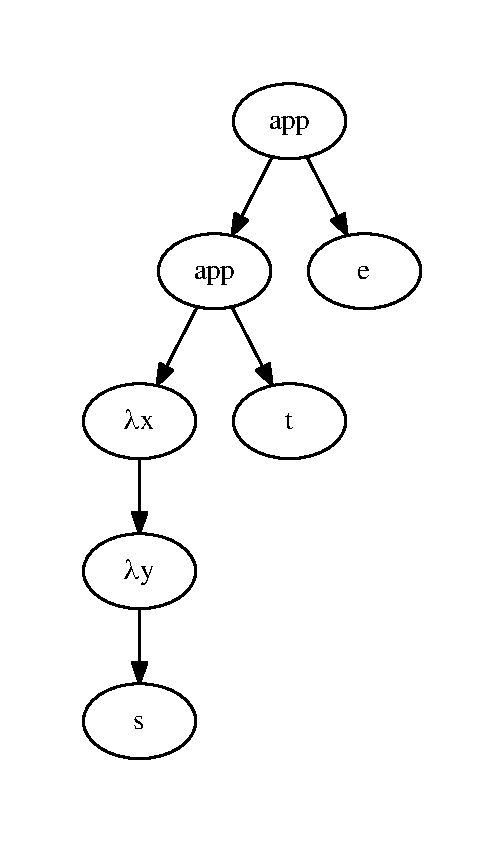
\includegraphics[width=4cm]{measure_ce1.pdf}
%     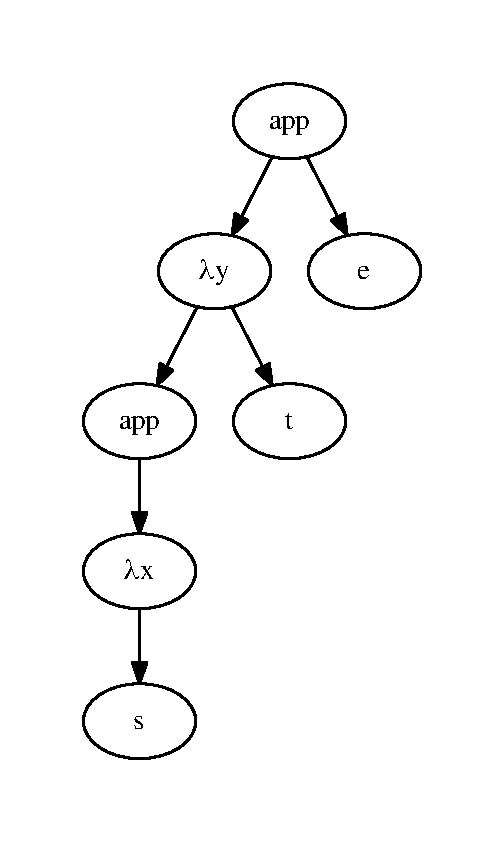
\includegraphics[width=4cm]{measure_ce2.pdf}
%   \end{center}
%
% The weight of the abstraction on $x$ decreases as expected, but at the same time
% the weight of the abstraction on $y$ increases. Since $y$ is higher, its weight
% contributes more.
%

\section{Some semantical definitions taken from ``Specifying Systems''}

\subsection{Alpha-renaming during instantiation (ch. 17.5.8)}
\todo[inline]{Fill in}

\subsection{Parametrized Instance (ch. 17.5.5) }
We consider the meaning of the statement

$$I(p_1,\ldots,p_m) == \INSTANCE N\;\WITH q_1 \iwith e_1, \ldots,q_n \iwith
  e_n$$

where $N$ is a module, $q_1,\ldots,q_n$ are declared constants/variables in $N$
 and $p_1,\ldots,p_m$ are fresh formal parameters\footnote{The book speaks of
   constants not occcurring in $N$ instead.}. Let $Op(r_1,\ldots,r_p) = e$ be a
 definition in $N$. Then its instance $I!Op$ is defined as

$$I!Op(p_1,\ldots,p_m,r_1,\ldots,r_p) == \overline{e}$$

where $\overline{e}$ has approriately alpha-renamed primed variables in the
 context of $\ENABLED$.

If the module has only constant declarations, no levels have to be checked.
 Otherwise, the level of the instantiation term $e_i$ may not be larger than
 the level of the declared operator $p_i$ it is replacing.


\end{document}
